\documentclass{article}
\usepackage[utf8]{inputenc}
\usepackage{graphicx}
\usepackage{booktabs}
\usepackage{amsmath}
\usepackage{amssymb}
\usepackage[margin=1in]{geometry}
\usepackage{hyperref}
\usepackage{xcolor}

\title{The Verifiability Gap:\\ Evaluation Depth Bounds Self-Improvement in Physical Design}
\author{Anonymous submission}
\date{}

\newcommand{\pending}[1]{\textcolor{gray}{[#1]}}

\begin{document}
\maketitle

\begin{abstract}
Self-improving systems are commonly credited with whatever their own evaluator
reports. We ask how much of a self-improvement loop's apparent progress survives
when the evaluation is made stronger, and we build the measurement in a domain with
a hard external ground truth: physical design. A placement can be scored in seconds
on the placer's internal estimate, in minutes on the legalized placement, or on a
trial route, or on timing. We instrument an industrial-grade open-source flow so
that every candidate placement is scored at every rung of this ladder, with a cost
ledger and a frozen protocol. Three findings. First, skipping legalization does not
merely make the score optimistic: it inverts the ranking. The pre-legalization
wirelength signal is anti-correlated with the legalized wirelength
($\rho=-0.89$, 32 designs) and with congestion ($\rho=-0.92$), and selecting on it
costs $19.7\%$ of wirelength and $124.7\%$ of congestion against what was available
in the same candidate pool; on an external commercial yardstick the choice it makes
is worse on 31 of 32 designs. Second, a loop driven by that signal ends half a
pool-step \emph{worse} than it started in $90$--$93\%$ of 800 trajectories while
reporting a $+1.22$ believed improvement, and its true-improvement horizon is
$r^\star=0$. Third, the same structural problem recurs one rung up: legalized
wirelength itself anti-ranks setup slack ($\rho=-0.47$). We then give an
evaluation-budget method that beats the best fixed-rung strategy at every budget
tested by $0.071$--$0.089$ rank, and whose preference transfers across process
technologies with rank correlation $0.87$--$0.91$. A live implementation of the same
loops reproduces the ordering and the horizon, and on held-out splits, including six
sealed designs that were used for nothing but the report, the unfaithful arm is negative
and the faithful arms positive in every split. We do not claim accelerating
self-improvement; the claim is about what bounds it.
\end{abstract}

\section{Introduction}

Recursive self-improvement research has produced working systems that improve their
own prompts, data, code, or training procedure. The strongest claims --- that the
improver itself gets better, and gets better faster --- remain unsupported. A
recurring reason is methodological: in most testbeds the signal the system optimizes
is the signal used to judge it, so a loop that has learned to satisfy its evaluator
is indistinguishable from a loop that has improved.

We take the position that the missing instrument is a testbed where the evaluator and
the truth are separated by a measurable, priced ladder. Physical design is such a
domain. A placement can be evaluated at very different depths: the placer's internal
wirelength estimate in seconds, computed on a placement whose cells are not yet
aligned to the site grid; the wirelength of the legalized, detailed placement in tens
of seconds; the same plus real congestion from a trial route in minutes; plus timing
and DRC in hours. Each rung costs more and sees more, and each is a plausible thing
for an autonomous agent to optimize, because agents are routinely run under a budget.

\paragraph{Contributions.}
(i) A formalization of a self-improvement loop in which verifier error is written into
the persistent state and therefore compounds, with a proposition predicting a finite
true-improvement horizon $r^\star$ when the verifier is imperfect and true returns
diminish (\S\ref{sec:model}).
(ii) An instrumented, reproducible testbed: 32 designs across four process
technologies, a leveled verifier, a per-candidate cost ledger that separates the
loop's evaluation cost from measurement overhead, and a frozen protocol with a dated
amendment trail (\S\ref{sec:testbed}).
(iii) A measurement of verifier fidelity per rung: the cheap signals anti-rank the
truth, and the cost of selecting on them is quantified internally and confirmed
externally (\S\ref{sec:stage1}, \S\ref{sec:external}).
(iv) A measurement of the gap over rounds and of the horizon $r^\star$
(\S\ref{sec:dynamics}), including the observation that the ruler is a rung too
(\S\ref{sec:timing}).
(v) An evaluation-budget method with a measured margin and a cross-technology
transfer test (\S\ref{sec:method}, \S\ref{sec:transfer}).

\section{Related work}

\paragraph{Self-improvement systems.} GEPA and Meta-Harness optimize prompts and
harness code from execution traces; SEAL and Absolute Zero extend self-improvement to
generated data and self-edit strategies; the Darwin Godel Machine and Godel Agent
modify their own code and keep a lineage of versions; Hyperagents and MetaRSI place
the improver itself inside the optimization and report that the meta level can improve
and transfer. Reviews and METR's analysis observe that evidence for accelerating
self-improvement is thin and that the field lacks agreement on what counts as a
demonstration. Our relationship to that work is complementary and deliberately
adversarial: we do not propose another improver, we supply the instrument these
systems lack and use it to measure how much of a reported gain is evaluation depth.

\paragraph{Multi-fidelity optimization.} Racing, successive halving, Hyperband and
multi-fidelity Bayesian optimization trade cheap evaluations for accuracy under a
budget. Our setting differs in one respect that matters for the conclusion: there, a
noisy objective costs a per-round loss; here the accepted edit is written into the
improver's persistent state and is reused as the basis of the next proposal, so the
ceiling we derive comes from accumulation rather than from variance.

\paragraph{Physical design.} Placement flows already rely on staged evaluation, and
practitioners know that early-stage proxies mislead: the flow's own tooling refuses
to score unlegalized placements for congestion because overlapping cells fake a low
overflow. What has not been done is to quantify, per rung, how badly the proxy ranks
the truth, on a large design set, with the cost of each rung accounted.

\section{Formalization}
\label{sec:model}

\textbf{Definition 1 (self-improvement loop).} A loop is a tuple $(S,P,V,U)$: a state
$S$ that persists across rounds, a proposer $P$ that emits a candidate edit, a
verifier $V$ that decides acceptance, and an update $U$ that writes accepted edits into
$S$. Strong self-improvement is the case where $S$ describes $(P,V,U)$ itself.

\textbf{Definition 2 (verifier rung).} A rung is a pair (signal, cost). Rung order is
by cost. Rung $v$ is \emph{sound} to the extent that its ordering of candidates agrees
with the truth ordering.

\textbf{Definition 3 (verifier fidelity).} Precision $p(v)$ is the fraction of edits
accepted by rung $v$ whose true objective is not worse; rank fidelity $\rho(v)$ is the
Spearman correlation between the rung's signal and the true objective on a common
candidate pool.

\textbf{Definition 4 (headline quantities).} For a loop at round $r$ holding state
$S_r$, let $dQ_V(r)$ be the improvement of the rung signal from its start and
$dQ_T(r)$ the improvement of the true objective. The verifiability gap is
$VG_r = dQ_V(r) - dQ_T(r)$, and the true-improvement horizon $r^\star$ is the smallest
$r$ after which $dQ_T$ is never positive again.

\paragraph{Model.} Assume (i) beneficial edits yield diminishing true returns $g(r)$,
concave and decreasing to zero; (ii) harmful edits that the verifier accepts cost $c$
and remain in the state, so their damage accumulates; (iii) the verifier accepts a
beneficial edit with probability $p$ and a harmful edit with probability $f$. Then
\begin{equation}
\mathbb{E}[dQ_T(r)] \;=\; p\,g(r) \;-\; (1-p)\,c\,A(r),
\end{equation}
where $A(r)$ counts absorbed harmful edits and grows with $r$.

\paragraph{Proposition 1.} For any $p<1$, with $g$ concave and decreasing to zero and
$A(r)$ non-decreasing, $\mathbb{E}[dQ_T(r)]$ is maximised at a finite $r^\star$, and
$dr^\star/dp > 0$. If the rung signal does not saturate, $VG_r$ grows without bound on
the same run.

The measurable predictions are: a finite interior horizon for weak rungs; an ordering
of $r^\star$ across rungs that tracks measured fidelity; and a larger gap for a proxy
calibrated on a different process.

\section{Testbed and protocol}
\label{sec:testbed}

\paragraph{Flow.} iEDA at a frozen revision, built in an isolated workspace, with the
placement substage exposed as a per-candidate pipeline: global placement with knobs
(target density, congestion effort, seed), then legalization and detailed placement,
then optional trial-route congestion, then optional placement timing.

\paragraph{Designs.} 32 of 35 registry entries are usable; three are excluded because
their references point at dead temporary paths or a foreign source tree, and they are
listed rather than dropped silently. The set spans four process technologies.

\paragraph{Verifier rungs.}
\begin{center}
\begin{tabular}{llll}
\toprule
rung & signal the loop sees & legalized & charged cost \\
\midrule
V0 & placer-internal wirelength & no & global placement \\
V0b & solver-internal route utilization & no & global placement \\
V1u & DEF wirelength at the legalizer input & no & global placement \\
V1 & wirelength of the legalized placement & yes & placement + legalization \\
V2 & V1 plus trial-route congestion (Pareto) & yes & plus trial route \\
V3 & V2 plus placement timing & yes & plus a timing pass \\
\bottomrule
\end{tabular}
\end{center}

\paragraph{Truth and why we do not scalarize.} The fair ruler is the pair (legalized
wirelength, trial-route congestion union), computed by one shared evaluator used by
every arm; the evaluator refuses unlegalized candidates, as the flow's own tooling
does. Because the two components have very different dynamic ranges, any weighted sum
would be dominated by congestion and the conclusion would depend on the weight. We
therefore do not scalarize: in-loop acceptance of the strongest rung uses Pareto
dominance, and offline scoring uses percentile ranks inside the candidate pool, so
believed and true curves live on one scale without an arbitrary weight.

\paragraph{Cost accounting.} Every candidate evaluation appends one record carrying
the measured wall and CPU seconds of each stage plus the identity of the loop that
requested it. A rung is charged exactly the stages it needs, and the cost of computing
the truth is never charged to the loop.

\paragraph{Anti-self-deception.} The protocol fixes the truth instrument in advance,
refuses unlegalized candidates, rebuilds each candidate work directory fresh, compares
rungs on identical candidates, and requires a cost record for every run. Six defects
were found and fixed during the campaign and are recorded as dated amendments rather
than quietly repaired, including two that produced results which looked plausible
rather than results which broke: a concurrency race in which two loops could share a
work directory, and failures cached as results.

\section{How well does each rung rank the truth}
\label{sec:stage1}

\paragraph{Setup.} 29 candidates per design on a grid of target density
$\{0.55,\dots,0.95\}$ crossed with congestion effort $\{0,3,7\}$ plus replicate seeds,
on 32 designs: 928 candidate evaluations, 0 failures. Every candidate is scored by
every rung and by the truth.

\begin{center}
\begin{tabular}{lcc}
\toprule
rung & vs legalized wirelength & vs congestion union \\
\midrule
V0 internal wirelength & $-0.892\,[-0.841,-0.596]$ & $-0.918\,[-0.896,-0.788]$ \\
V1u unlegalized DEF wirelength & $-0.891\,[-0.839,-0.589]$ & $-0.922\,[-0.895,-0.784]$ \\
V0b solver route utilization & $+0.682\,[+0.532,+0.723]$ & $+0.737\,[+0.570,+0.737]$ \\
V1 legalized wirelength & $+1.000$ & $+0.970\,[+0.699,+0.932]$ \\
V2 fair ruler & $+0.976\,[+0.791,+0.926]$ & $+0.999\,[+0.965,+0.997]$ \\
\bottomrule
\end{tabular}
\end{center}

\paragraph{Finding 1 (the inversion).} The two pre-legalization wirelength signals are
not noisy versions of the truth: they are anti-correlated with it at about $-0.89$,
with intervals excluding zero by a wide margin. The mechanism is measurable and
boring, which is why it is dangerous: legalization must displace cells by an amount
that grows with how tightly the placer packed them, so the pre-legalization score
rewards exactly the candidates whose advantage evaporates afterwards. On one design
the legalizer move alone costs $13\%$ of wirelength at target density $0.95$ and $2\%$
at $0.60$.

\paragraph{Finding 2 (the distrusted signal is the informative one).} The solver
route utilization, which the project's own tooling flags as not trustworthy, is
positively correlated with true congestion ($+0.74$). We report the measurement.

\begin{figure}[t]
\centering
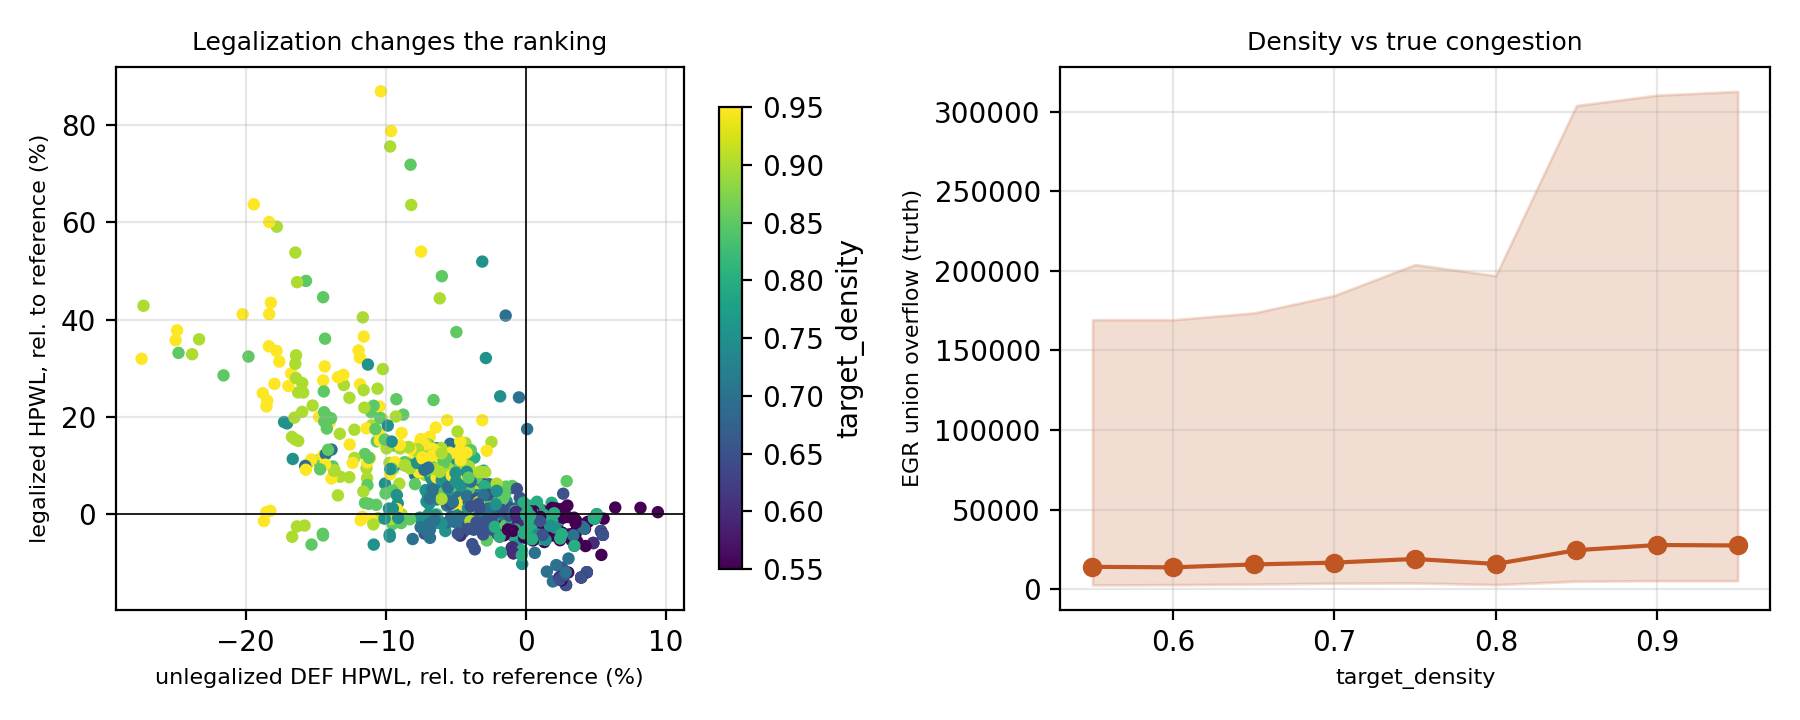
\includegraphics[width=\linewidth]{figures/fig3_mechanism.png}
\caption{The mechanism. Left: legalization changes the ranking of candidates.
Right: true congestion grows with target density, so a score that rewards density
rewards the wrong direction on this axis.}
\end{figure}

\begin{center}
\begin{tabular}{lcc}
\toprule
rung & legalized wirelength regret & congestion regret \\
\midrule
V0 & $+19.7\%\,[+18.8,+32.7]$ & $+124.7\%\,[+128.6,+700.6]$ \\
V1u & $+19.7\%\,[+19.0,+33.8]$ & $+125.5\%\,[+131.7,+715.0]$ \\
V0b & $+0.6\%$ & $+0.7\%$ \\
V1 & $0.0\%$ & $0.0\%$ \\
\bottomrule
\end{tabular}
\end{center}

\begin{figure}[t]
\centering
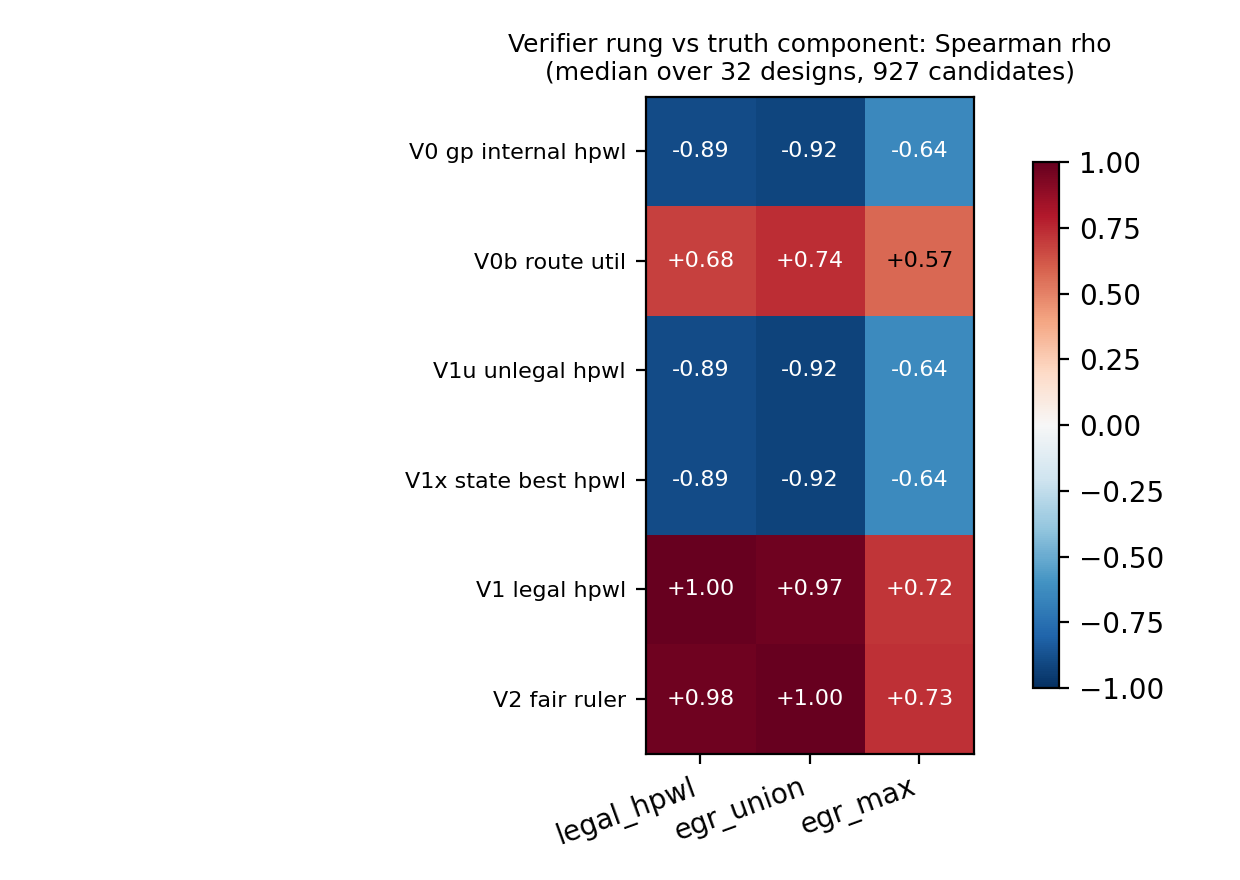
\includegraphics[width=\linewidth]{figures/fig1_fidelity_heatmap.png}
\caption{Spearman correlation between each verifier rung and each truth component,
median over 32 designs with bootstrap intervals. The pre-legalization rungs are
anti-correlated with the truth.}
\end{figure}

\begin{figure}[t]
\centering
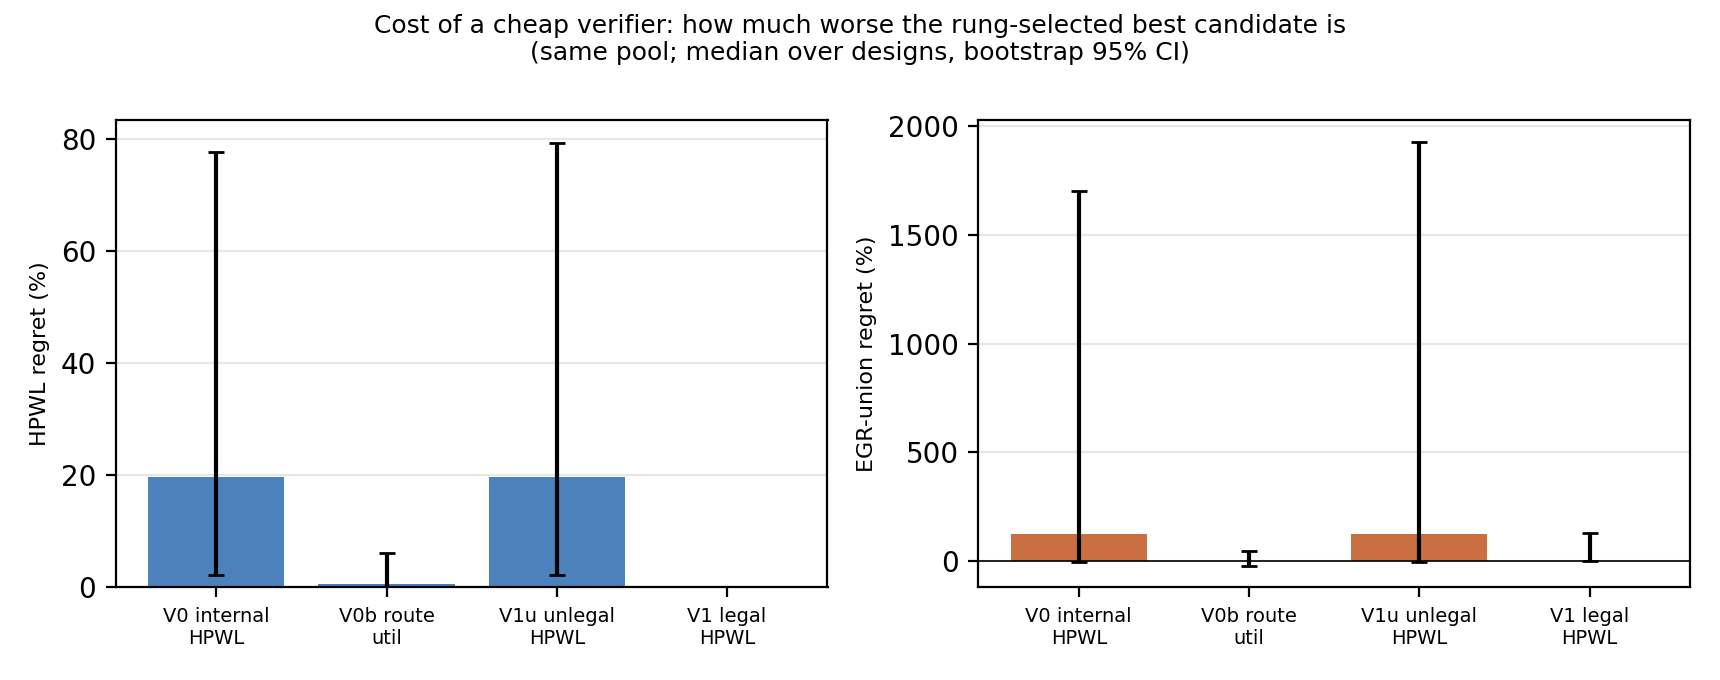
\includegraphics[width=\linewidth]{figures/fig2_selection_regret.png}
\caption{Cost of a cheap verifier: how much worse the rung-selected best candidate is
than the truth-selected best candidate of the same pool.}
\end{figure}

\paragraph{Finding 3 (the price of a cheap verifier).} Selecting on the
pre-legalization signal costs about $20\%$ of legalized wirelength and $125\%$ of
congestion relative to what was available in the same pool. We also note that $66\%$
of designs place their truth-best candidate on the density floor, verified to be a
plateau rather than an artifact of the grid, and we state that rather than presenting
it as an interior optimum.

\section{The ruler is a rung too}
\label{sec:timing}

If the ladder is real, the quantity we have been calling the truth must itself be a
proxy for the rung above it. We test this by adding placement timing (a physical
timing evaluation with an HPWL-based pre-route RC model) as a third truth component,
over 24 designs and 696 candidates.

\begin{center}
\begin{tabular}{lcc}
\toprule
signal & vs setup TNS & vs setup WNS \\
\midrule
V0 internal wirelength & $+0.219\,[+0.025,+0.426]$ & $+0.112$ \\
V1u unlegalized DEF wirelength & $+0.216\,[+0.024,+0.425]$ & $+0.122$ \\
V1 legalized wirelength & $\mathbf{-0.471\,[-0.574,-0.202]}$ & $-0.261\,[-0.393,-0.069]$ \\
fair ruler (wirelength + congestion) & $-0.247\,[-0.502,-0.092]$ & $-0.227$ \\
\bottomrule
\end{tabular}
\end{center}

\paragraph{Finding 4.} The fair ruler, and especially its wirelength component, is
negatively correlated with timing: within a design, the candidates that look best on
legalized wirelength
tend to be worse on setup slack, and vice versa. The geometry-best candidate is also
the timing-best on 7 of 24 designs. The magnitude is modest (selecting on geometry
costs a median $6.7\%$ of TNS relative to the timing-best candidate) but the sign is
systematic and the interval excludes zero.

\begin{figure}[t]
\centering
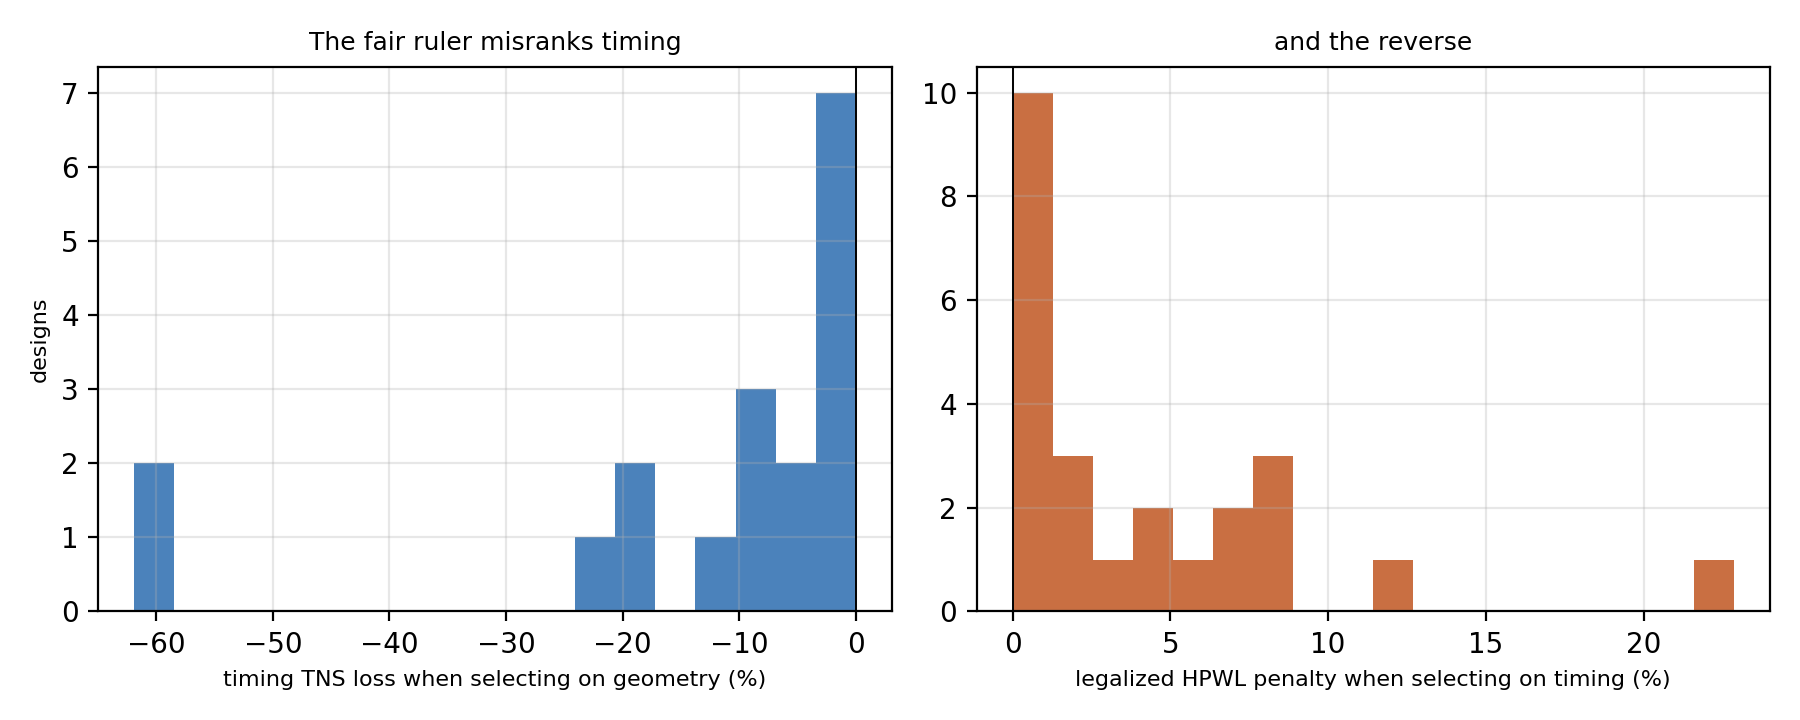
\includegraphics[width=\linewidth]{figures/fig6_timing_vs_ruler.png}
\caption{The fair ruler misranks timing, and the reverse: selecting on geometry
costs setup slack, selecting on timing costs wirelength.}
\end{figure}

\paragraph{Interpretation, stated carefully.} This timing is a pre-clock-tree
evaluation with a wireload model, so it is itself a proxy for signoff timing; we are
not claiming to have reached signoff. What the measurement establishes is the
structural point: every rung we have measured is a proxy for the next, and a proxy can
\emph{invert} the ordering of the rung above rather than merely add noise to it.
Optimizing the wrong rung therefore does not cost a little accuracy; it moves the
design in the wrong direction, and a loop accepting that signal will do so
persistently.

\subsection{A signoff spot check}

The rungs above the ruler are clock tree synthesis, routing and DRC, where a candidate
costs minutes to tens of minutes rather than seconds. We therefore ran the chain as a
spot check: the geometry-optimal candidate and the candidate the cheap rung is
attracted to, both for one design, pushed from the placed DEF through clock tree
synthesis, routing and DRC with the same flow and configuration.

\begin{center}
\begin{tabular}{lcc}
\toprule
candidate & routing wall time & DRC violations \\
\midrule
geometry-optimal (density 0.65, effort 7) & 148\,s & 155 \\
cheap-rung attractor (density 0.95, effort 0) & 1619\,s & 332 \\
\bottomrule
\end{tabular}
\end{center}

Both route to completion. The cheap verifier's pick takes eleven times longer to route
and ends with 2.1 times as many DRC violations. This is the direction the ladder
predicts, observed at the end of the flow rather than on a proxy. We state the scope
plainly: one design and two candidates, an illustration that the ordering survives to
signoff rather than a measurement with a sampling distribution, and nothing else here
depends on it. At roughly twenty-five minutes per candidate under load, a
campaign-wide signoff rung would cost about a hundred times the geometry ladder.

\section{Dynamics: the gap over rounds and the horizon}
\label{sec:dynamics}

\paragraph{Design.} Every rung runs an identical adaptive search over (density,
effort, seed) for 16 rounds from the same start candidate, on 32 designs and 5 seeds:
800 trajectories. The loop sees only its rung's signal and is charged that rung's
measured cost. The harness scores every held state with the truth, which the loop
never sees. Two implementations are reported: a \emph{replay} over the candidate pool
that Section 5 already evaluated, which is exactly deterministic and paired across
rungs, and a \emph{live} run through fresh placements as corroboration. The replay is
primary because pairing is what makes a comparison of rungs meaningful.

\begin{center}
\begin{tabular}{lcccccccc}
\toprule
rung & cost (s) & true gain & worse & $VG$ at $r{=}16$ & $r^\star$ & interior $r^\star$ & gain/s \\
\midrule
V0 internal wirelength & 162 & $-0.482$ & $93\%$ & $+1.218$ & 0 & 34\% & $-2.2\text{e-}3$ \\
V1u unlegalized wirelength & 172 & $-0.500$ & $90\%$ & $+1.232$ & 0 & 39\% & $-1.9\text{e-}3$ \\
V0b route utilization & 154 & $+0.071$ & 28\% & $+0.018$ & 3 & 68\% & $2.1\text{e-}4$ \\
V1 legalized wirelength & 188 & $+0.161$ & 10\% & $+0.018$ & 4 & 85\% & $6.4\text{e-}4$ \\
V2 fair ruler (Pareto) & 269 & $+0.143$ & 10\% & $0.000$ & 3 & 83\% & $4.4\text{e-}4$ \\
\bottomrule
\end{tabular}
\end{center}

\paragraph{Finding 5 (the gap is not noise).} A loop driven by the pre-legalization
signal does not merely fail to improve: it ends half a pool-step \emph{worse} than
where it started, in $90$--$93\%$ of trajectories, while reporting a believed
improvement of $+1.22$ rank points. A faithful verifier has essentially no gap
($+0.018$).

\paragraph{Finding 6 (the horizon).} For both cheap rungs the median $r^\star$ is $0$:
the truth peak is the starting state, i.e.\ every accepted edit was net harmful, and
this is an interior result in $34$--$39\%$ of trajectories. For faithful rungs
$r^\star$ is 3--4 with an interior optimum in $68$--$85\%$, the ordinary behaviour of
a working search. The model predicts exactly this ordering.

\paragraph{Finding 7 (the mechanism, measured directly).} Absorption rate is the
share of accepted edits that a stronger verifier confirms: the fraction of the
persistent state's updates that were genuine improvements rather than damage. It is
exactly the quantity the model's second assumption is about.

\begin{center}
\begin{tabular}{lccc}
\toprule
rung & accepted & of which harmful & AR (confirmed share) \\
\midrule
V0 internal wirelength & 5.0 & 3.0 & 0.33 \\
V1u unlegalized wirelength & 5.0 & 4.0 & 0.33 \\
V0b route utilization & 3.0 & 1.0 & 0.60 \\
V1 legalized wirelength & 3.0 & 1.0 & 0.67 \\
V2 fair ruler (Pareto) & 3.0 & 1.0 & 0.69 \\
\bottomrule
\end{tabular}
\end{center}

The decomposition of Proposition~\ref{sec:model} is measurable, so we account for it
rather than fitting a curve: every accepted edit is classified by whether the truth
improved or worsened, and the two contributions are summed. The identity
$\text{net} = \text{confirmed gain} - \text{harmful loss}$ holds exactly on every
trajectory by construction.

\begin{center}
\begin{tabular}{lccccc}
\toprule
rung & confirmed gain & harmful loss & net & confirmed accepts & harmful accepts \\
\midrule
V0 internal wirelength & $+0.214$ & $\mathbf{+0.732}$ & $\mathbf{-0.496}$ & 2.0 & 3.0 \\
V1u unlegalized wirelength & $+0.227$ & $\mathbf{+0.732}$ & $\mathbf{-0.482}$ & 2.0 & 3.0 \\
V0b route utilization & $+0.451$ & $+0.375$ & $+0.063$ & 2.0 & 1.0 \\
V1 legalized wirelength & $+0.527$ & $+0.295$ & $+0.152$ & 2.5 & 1.0 \\
V2 fair ruler (Pareto) & $+0.554$ & $+0.339$ & $+0.170$ & 2.0 & 1.0 \\
\bottomrule
\end{tabular}
\end{center}

Three things happen at once with a weak verifier, and the table separates them.
First, the damage term dominates: for the cheap rungs the harmful loss is $3.4$ times
the confirmed gain, which is what makes the net negative, whereas for the faithful
rungs the confirmed gain is $1.6$--$1.8$ times the loss. Second, the gain term nearly
triples when the verifier becomes faithful ($0.214$ to $0.554$): a faithful verifier is
not merely more cautious, it finds better edits. Third, the damage term halves and
harmful accepts fall from three to one per trajectory while confirmed accepts stay near
two, so the weak verifier accepts more, and of worse quality. This is the compounding
mechanism made visible: the ceiling comes not from variance but from damage written into
the persistent state and then built upon.

\begin{figure}[t]
\centering
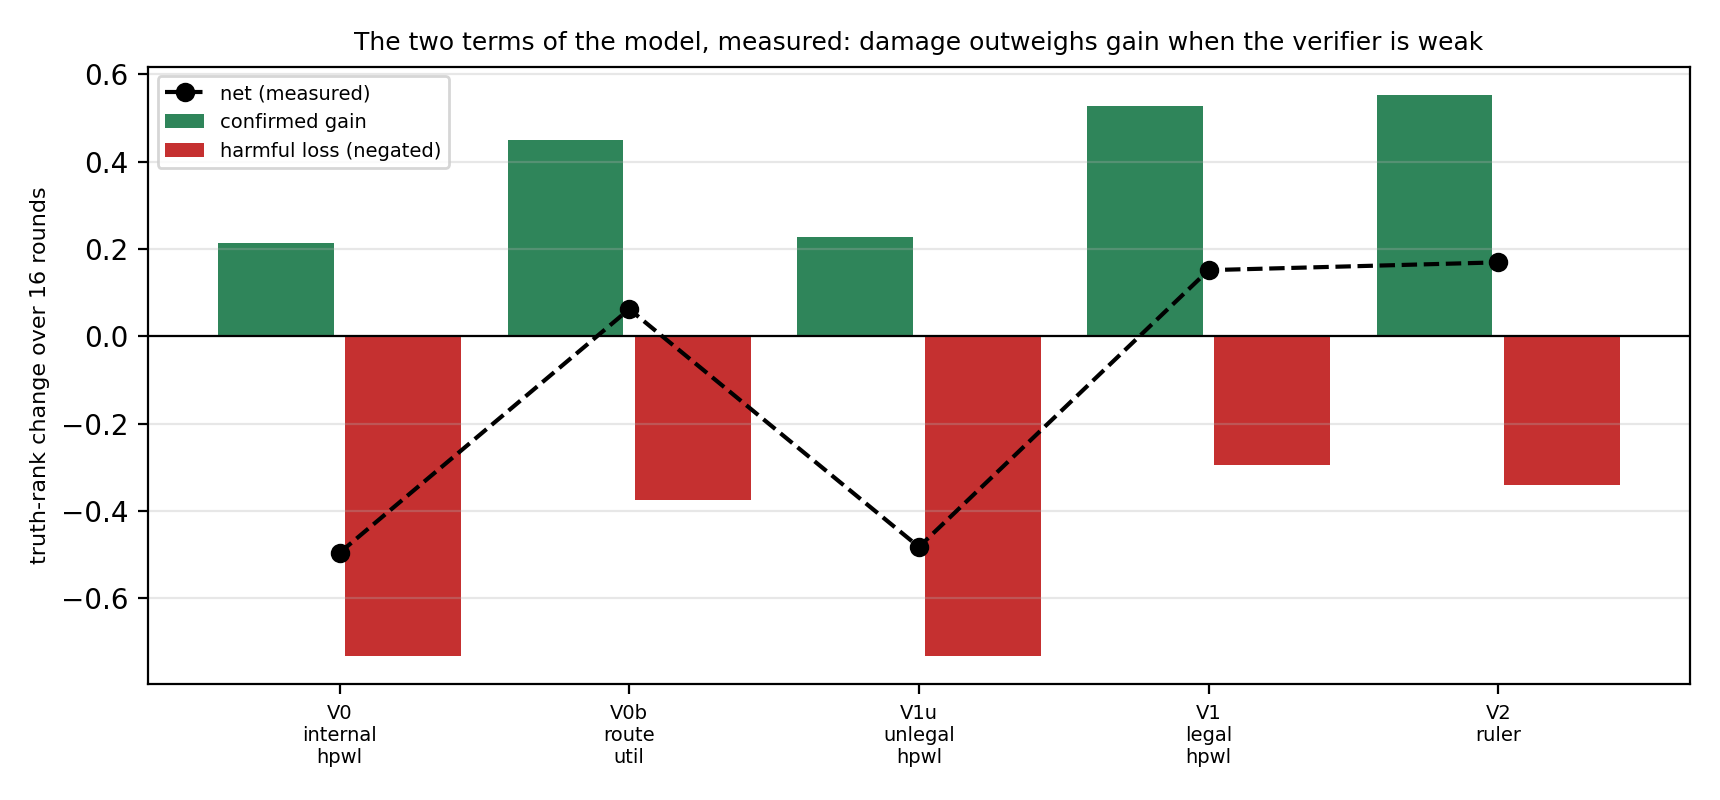
\includegraphics[width=0.95\linewidth]{figures/fig11_mechanism.png}
\caption{The two terms of the model, measured separately. Damage outweighs gain when
the verifier is weak, which is what makes the net truth change negative.}
\end{figure}

\paragraph{Finding 8 (what to pay for).} The true gain per second ranks V1
($6.4\text{e-}4$) above V2 ($4.4\text{e-}4$) above V0b ($2.1\text{e-}4$), with the
cheap rungs negative. The strongest rung costs $43\%$ more than the next one down and
returns slightly less. The value of a verifier is set by its fidelity per unit cost
with a saturation point, and the cheapest faithful rung is the best buy.

\begin{figure}[t]
\centering
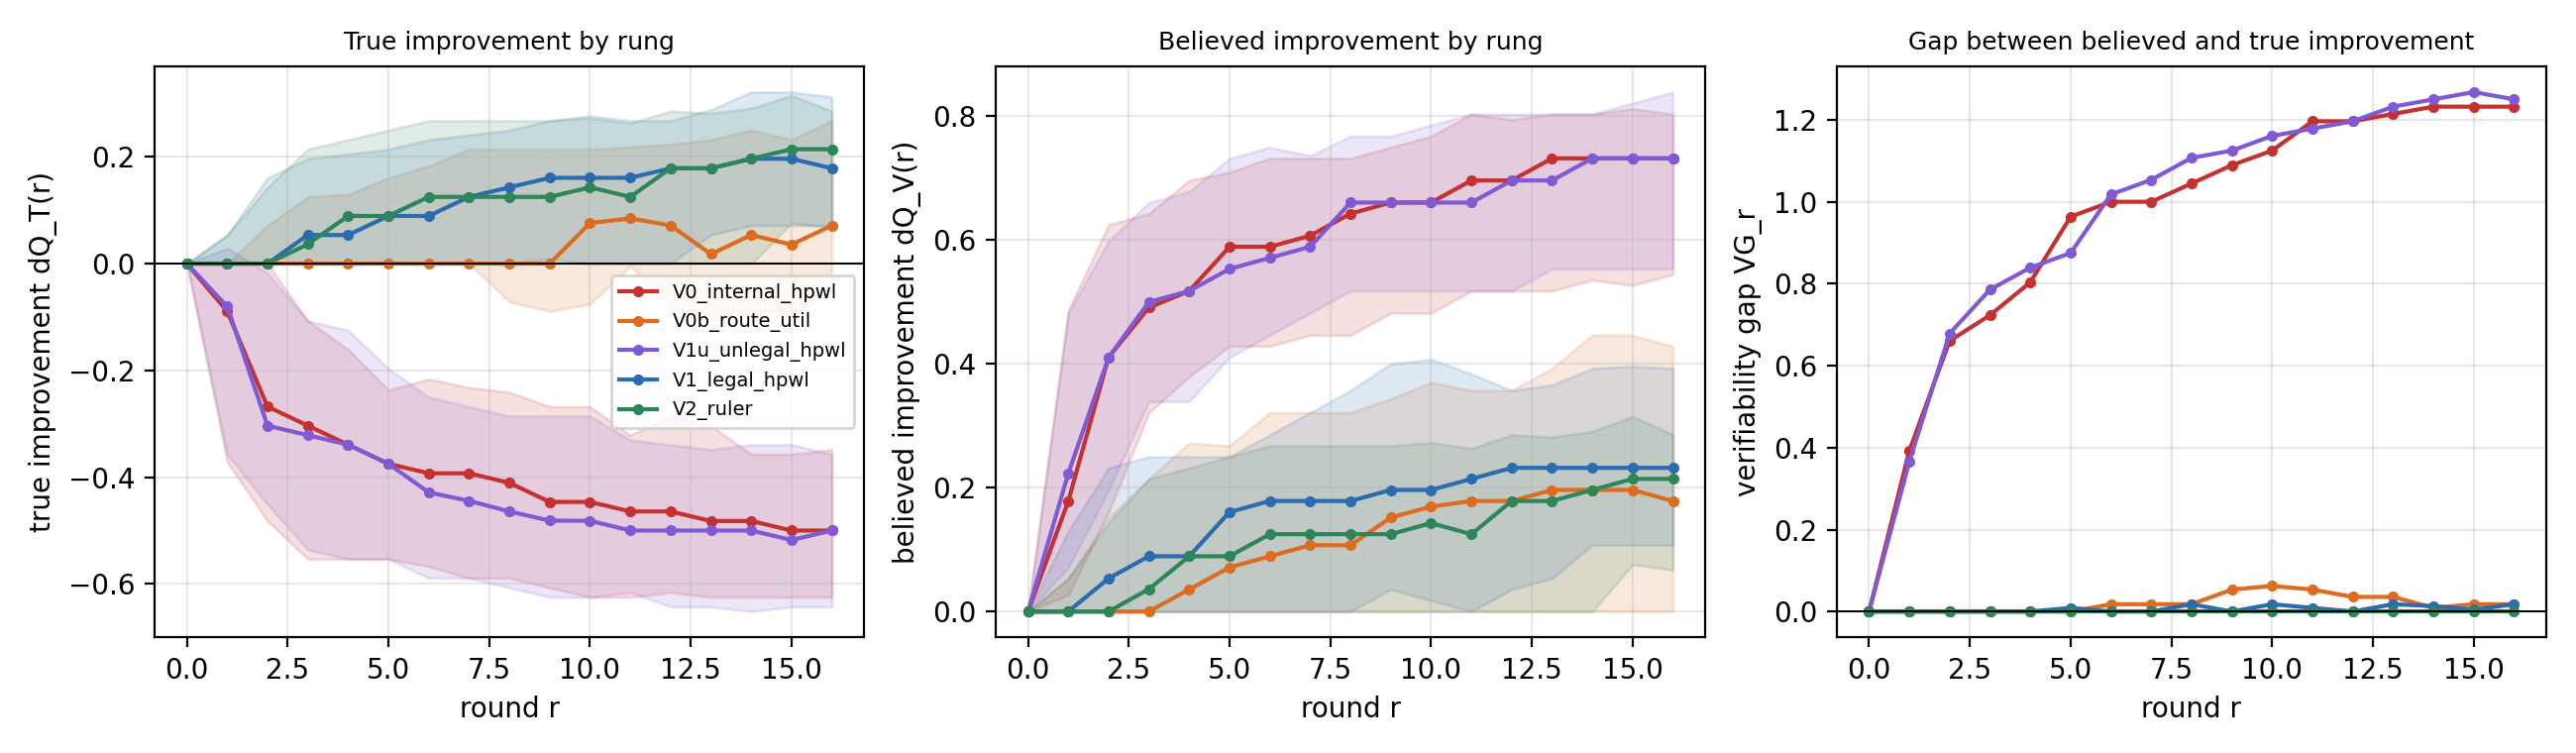
\includegraphics[width=\linewidth]{figures/fig4_dynamics.png}
\caption{Believed and true improvement by rung over 16 rounds, and the accumulated
verifiability gap. The cheap rungs' believed curves rise while their true curves
fall.}
\end{figure}

\subsection{Live corroboration (128 of 128 cells)}

The replay needs no solver time, which is also its weakness: it could describe the
pool rather than the loop. The live implementation drives the same four loops through
fresh placements and fresh truth evaluations, one loop per design per rung, 16 rounds
each, and the two are scored identically, by rank inside the pool the live run itself
explored.

\begin{center}
\begin{tabular}{lccccccc}
\toprule
rung & n live & live dQ\_T & replay dQ\_T & live $r^\star$ & replay $r^\star$ & live ends worse & replay ends worse \\
\midrule
V0 internal wirelength & 32 & $\mathbf{-0.699}$ & $-0.491$ & 0 & 0 & 97\% & 100\% \\
V1u unlegalized wirelength & 32 & $\mathbf{-0.644}$ & $-0.500$ & 0 & 0 & 100\% & 88\% \\
V1 legalized wirelength & 32 & $+0.175$ & $+0.143$ & 4 & 2 & 16\% & 9\% \\
V2 fair ruler (Pareto) & 32 & $+0.159$ & $+0.107$ & 4 & 2 & 16\% & 9\% \\
\bottomrule
\end{tabular}
\end{center}

The two implementations agree on what matters. The rungs split into the same two groups
in both: the cheap rungs are strongly negative and the faithful rungs positive. The
horizon is $r^\star=0$ for both cheap rungs in both, and the gap is large in both. On the
cheap rungs the live loop is worse than the replay and ends worse in 97--100\% of
trajectories, so the central claim is not an artifact of simulating the loop on a frozen
pool.

The one thing that is not stable is the order \emph{within} the cheap group: live puts V1u
above V0 while the replay puts V0 above V1u. The spread inside that group is $0.055$ live
and $0.009$ replayed, against a gap of about $0.8$ to the faithful group, so the two cheap
rungs are indistinguishable from each other and both are clearly separated from the
faithful pair. We report the boundary at the partition, not at a rank within the losing
group. The remaining differences (the live faithful arms gain slightly more, with a later
$r^\star$) are consistent with the live loop having a different pool to move through.

\begin{figure}[t]
\centering
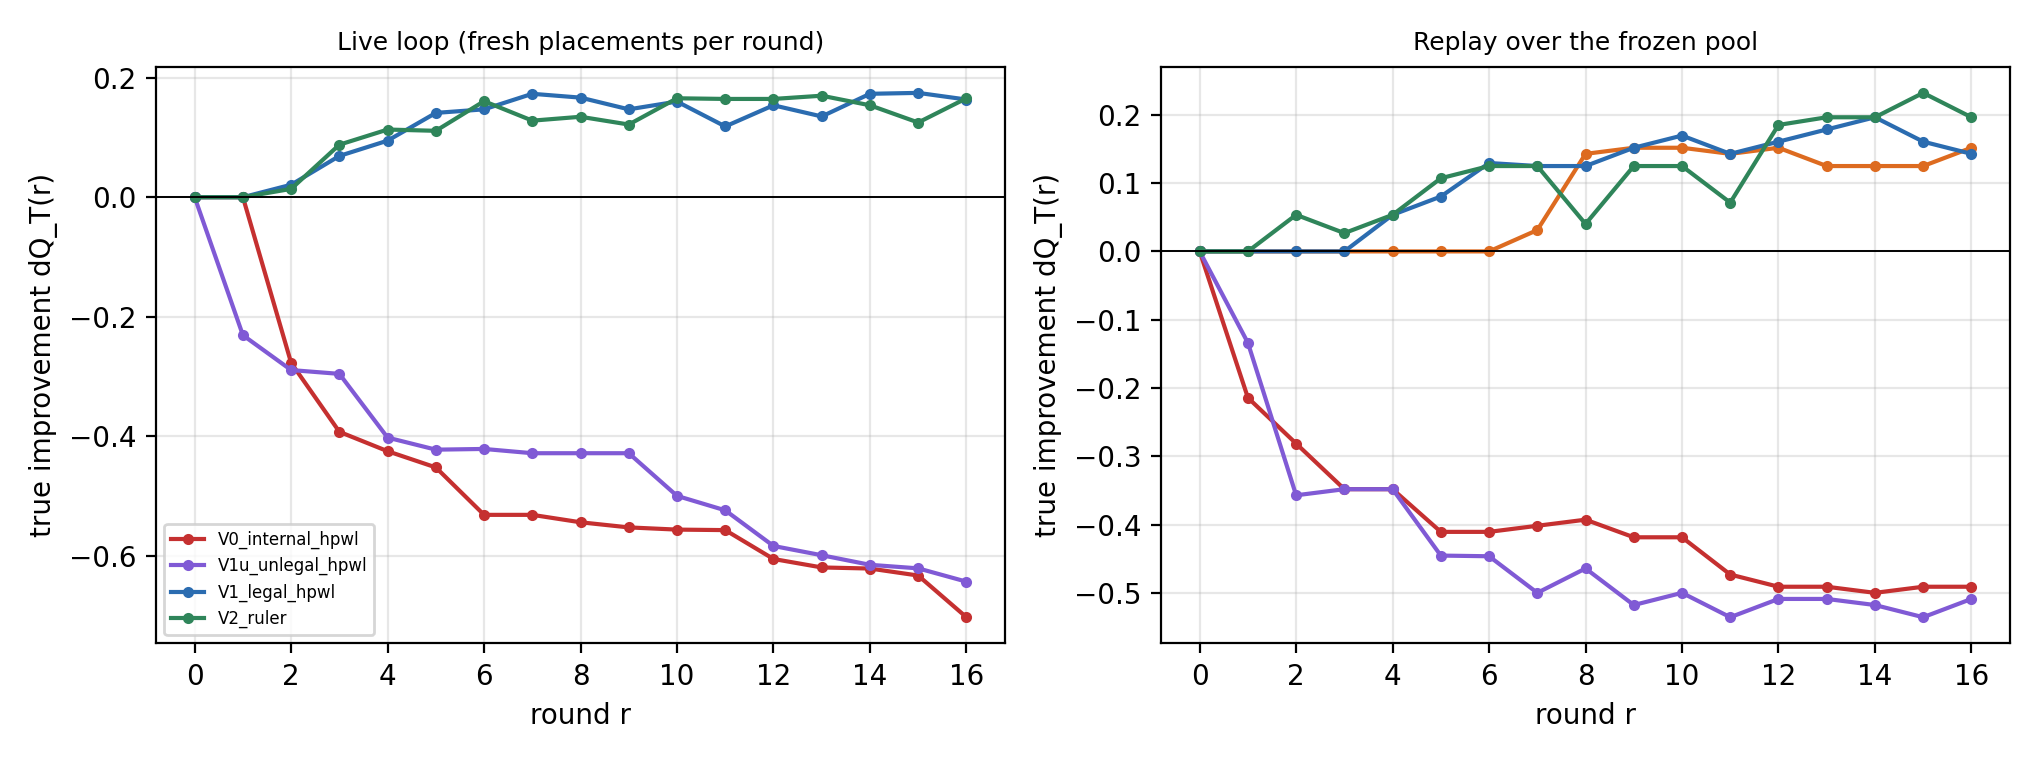
\includegraphics[width=\linewidth]{figures/fig10_live_vs_replay.png}
\caption{The same four loops run live (left) and replayed over the frozen pool
(right). The cheap rungs fall in both; the faithfulness ordering is preserved.}
\end{figure}

\section{What an evaluation budget should buy}
\label{sec:method}

Policies draw from the frozen pool, are charged the measured per-stage cost of every
evaluation, and their final placement is scored by the truth. Three families: climb on
a fixed rung; climb on the truth-shaped Pareto rule; and screen-then-confirm, which
draws $k$ candidates, ranks them with a screening rung, and confirms the best $m$ with
the strongest rung. Each policy is run under an explicit cost cap so policies compete
at equal budget.

\begin{center}
\begin{tabular}{lcccc}
\toprule
policy & 100\,s & 140\,s & 200\,s & 280\,s \\
\midrule
climb V0 (internal wirelength) & 0.143 & 0.125 & 0.107 & 0.109 \\
climb V1u (unlegalized wirelength) & 0.143 & 0.125 & 0.125 & 0.109 \\
climb V0b (route utilization) & 0.732 & 0.741 & 0.759 & 0.768 \\
climb V2 (fair ruler, Pareto) & 0.737 & 0.804 & 0.804 & 0.804 \\
climb V1 (legalized wirelength) & 0.804 & 0.804 & 0.839 & 0.839 \\
screen V0 then confirm V2 & 0.598 & 0.607 & 0.607 & 0.598 \\
screen V1u then confirm V2 & 0.607 & 0.625 & 0.625 & 0.616 \\
\textbf{screen V1 then confirm V2} & $\mathbf{0.893}$ & $\mathbf{0.893}$ & $\mathbf{0.911}$ & $\mathbf{0.920}$ \\
\bottomrule
\end{tabular}
\end{center}

\paragraph{Finding 9 (screening works, if the screening rung is faithful).} Ranking
with the cheapest faithful rung and confirming with the strongest wins at every
budget: $0.893$ against $0.804$ at $100\,$s and $0.920$ against $0.839$ at $280\,$s.
The advantage is not a cost effect, since it persists when the budget is doubled, so
screening buys breadth before commitment.

\paragraph{Finding 10 (screening on a wrong rung is worse than not screening).}
Screening with either pre-legalization signal lands at $0.60$, below climbing on a
faithful rung. A cheap screen is only cheap if it preserves the ordering it screens
on.

\paragraph{Finding 11 (the honest rule is the conservative one).} Climbing on the
Pareto ruler is worse than climbing on legalized wirelength alone ($0.804$ against
$0.839$) and never better: refusing any move that worsens the congestion component
gives up wirelength gains it could have kept.

\paragraph{Correction.} An earlier version of this section, on a pool of 16
design-seeds, reported the opposite conclusion, that screening does not beat a fixed
rung. That conclusion does not survive the full 32-design pool, where the screening
policy gains roughly nine rank points at every budget. The pre-registered kill
criterion was therefore evaluated on insufficient data and does not fire. We report
the reversal rather than quietly replacing it, because it is the campaign's own
illustration of the paper's thesis: a conclusion drawn on a small pool, evaluated by
one rung of evidence, was wrong.

\begin{figure}[t]
\centering
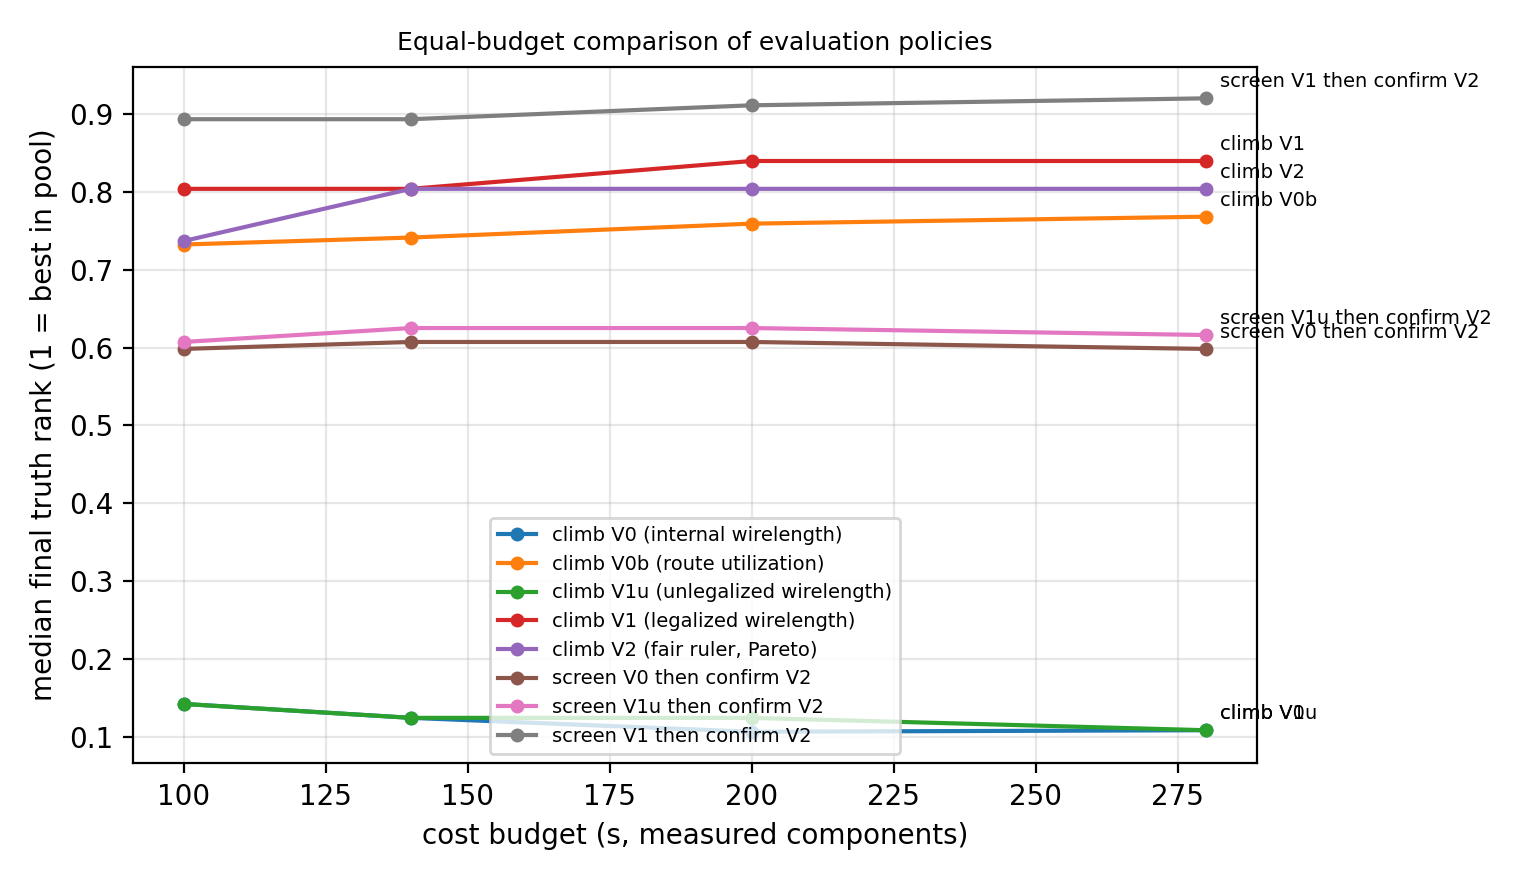
\includegraphics[width=0.85\linewidth]{figures/fig5_scheduling.png}
\caption{Equal-budget comparison of evaluation policies. Screening with a faithful
rung dominates at every budget; screening with an unfaithful one is near the bottom.}
\end{figure}

\subsection{Held-out splits, including the sealed designs}

The claims above were formed on the development split. Re-running the arms on the
validation, sealed and out-of-distribution splits tests whether they were fitted to the
designs that suggested them. The sealed designs were never used to choose a policy, a
threshold or a hyperparameter; the comparison below is a report, which is what the
protocol reserves them for.

\begin{center}
\begin{tabular}{llccccc}
\toprule
split & designs & n & A0 & A1 unleg. & A1 legal. & A2 ruler \\
\midrule
dev & 13 & 65 & 0.000 & $\mathbf{-0.500}$ & +0.179 & +0.125 \\
val & 5 & 25 & 0.000 & $\mathbf{-0.444}$ & +0.143 & +0.214 \\
sealed & 6 & 30 & 0.000 & $\mathbf{-0.536}$ & +0.125 & +0.125 \\
ood & 8 (other PDKs) & 40 & 0.000 & $\mathbf{-0.375}$ & +0.196 & +0.250 \\
\bottomrule
\end{tabular}
\end{center}

\paragraph{Finding 13 (the finding is not fitted to the designs that produced it).}
The sealed split reproduces the development result: the unfaithful arm destroys true
quality at about the same magnitude ($-0.536$ against $-0.500$), and the faithful arms
gain about the same amount. The out-of-distribution split, which differs in library,
cell height and routing stack, shows the same pattern again. The gain-per-second
ranking is stable too: on the sealed designs the legalized-wirelength arm gives
$8.5\text{e-}4$ per second against the ruler arm's $5.4\text{e-}4$ and the unlegalized
arm's negative value, the same ordering as on the development split.

Reading honestly, the sealed magnitudes differ from the development ones by up to about
a third, so the effect size is not precisely estimated at 30 trajectories per cell. What
is stable is the ordering and the sign, and that is what the paper claims.

\begin{figure}[t]
\centering
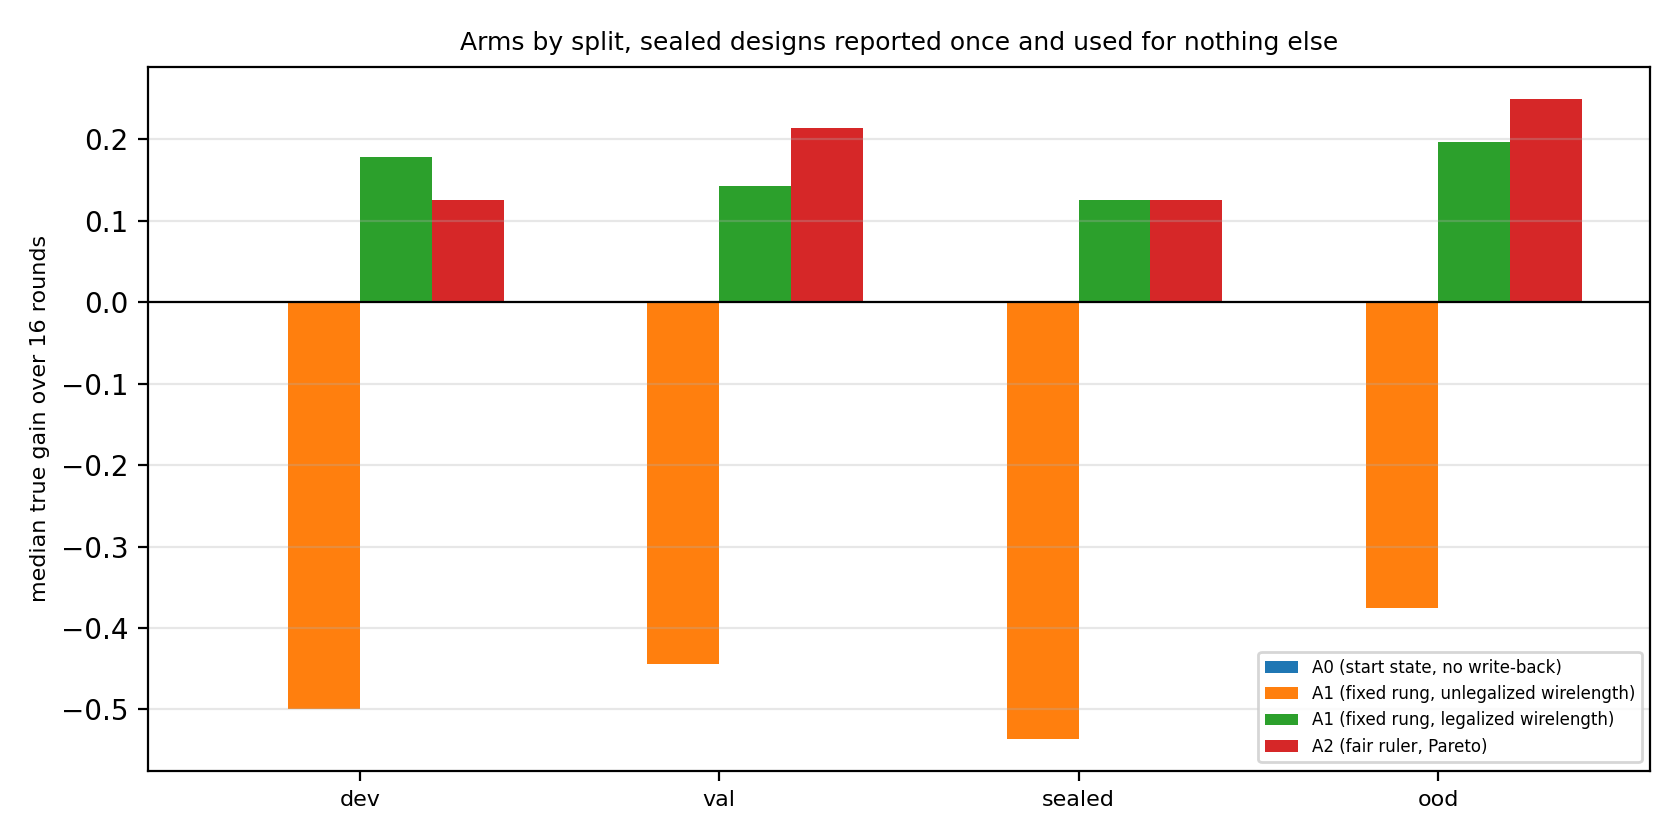
\includegraphics[width=0.92\linewidth]{figures/fig9_arms_by_split.png}
\caption{Arms by split. The sealed designs are reported once and used for nothing else;
the unfaithful arm is negative and the faithful arms positive in every split.}
\end{figure}

\section{External anchoring and transfer}
\label{sec:external}

\paragraph{External anchoring.} 32 designs carry a commercially placed reference DEF
for the same input DEF and floorplan. We score the reference, the ruler-optimal
candidate and the candidate the cheap rung is attracted to with the same independent
evaluator.

\begin{center}
\begin{tabular}{lcc}
\toprule
pick & wirelength / reference & congestion / reference \\
\midrule
ruler-optimal & $0.935$ & $1.228$ \\
cheap-rung (V0) attractor & $1.089$ & $2.902$ \\
\bottomrule
\end{tabular}
\end{center}

Paired across designs, the ruler-optimal pick is better than the cheap-rung pick on
31 of 32 designs for wirelength and 31 of 32 for congestion. The load-bearing
statement is the paired one, because it uses one external yardstick for both
policies. The absolute ratio is an anchor, not a like-for-like contest: the reference
was produced by a different tool with different settings and a different objective
mix, and our congestion is worse than the reference's overall. We therefore do not
claim to beat commercial tools; we claim that the choice the cheap verifier makes is
externally visible as worse, which is the same conclusion the internal analysis
reaches.

A note on cross-tool comparability, because it bounds what an absolute ratio can mean.
Our independent evaluator applied to the reference DEF agrees with the commercial tool's
own reported wirelength on only three of the four designs where both numbers exist, and
disagrees by $-21\%$ to $+9\%$ (aes 0.79, picorv32 0.86, apb4\_timer 0.91, s1238 1.09).
Two tools measuring wirelength for the same design differ by that much through fill
handling, unit conventions and what is counted. This is why the claim is built on a
paired comparison with one evaluator applied to both policies, and why we do not quote a
single absolute number as if it were tool-independent.

\begin{figure}[t]
\centering
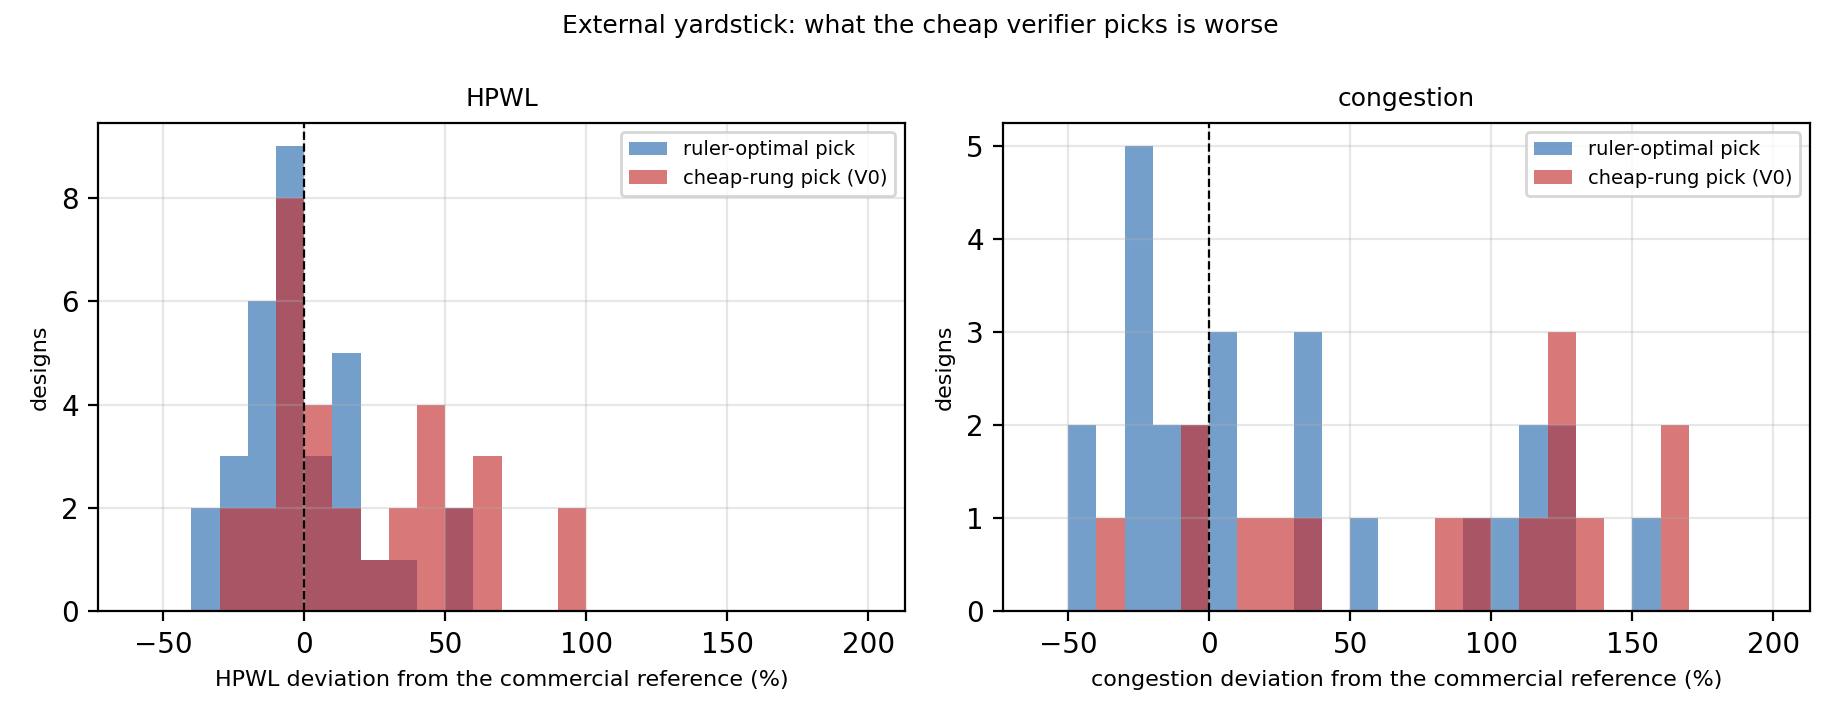
\includegraphics[width=0.9\linewidth]{figures/fig7_external_anchor.png}
\caption{Deviation from the commercial reference for the two pick policies. The
distribution of the cheap-rung pick is shifted to the right on both metrics.}
\end{figure}

\paragraph{Transfer.}\label{sec:transfer} The source domain is sky130 (24 designs); the targets are ics55
and nangate45 (four designs each), which differ in library, cell height and routing
stack. Every policy is run on every design at a fixed budget of $140\,$s.

\begin{center}
\begin{tabular}{lccc}
\toprule
policy & sky130 & ics55 & nangate45 \\
\midrule
climb V0 (internal wirelength) & 0.125 & 0.071 & 0.107 \\
climb V1u (unlegalized wirelength) & 0.098 & 0.125 & 0.116 \\
climb V0b (route utilization) & 0.714 & 0.777 & 0.746 \\
climb V1 (legalized wirelength) & 0.795 & 0.777 & 0.826 \\
climb V2 (fair ruler, Pareto) & 0.804 & 0.759 & 0.866 \\
screen V0 then confirm V2 & 0.661 & 0.379 & 0.513 \\
screen V1u then confirm V2 & 0.634 & 0.509 & 0.491 \\
screen V1 then confirm V2 & $0.902$ & $0.893$ & $0.799$ \\
\bottomrule
\end{tabular}
\end{center}

\paragraph{Finding 12.} The qualitative structure is identical in all three
technologies: both pre-legalization signals are the worst policies ($0.07$--$0.13$),
the faithful rungs are good ($0.71$--$0.87$), and screening with a faithful rung is
best or near-best ($0.80$--$0.89$). The Spearman correlation between the source and
target policy orderings is $0.874$ (ics55) and $0.905$ (nangate45), and applying the
source's choice on a target costs at most $8\%$ of the achievable rank. Which verifier
is worth using is determined by whether its signal is aligned with the truth, and that
alignment is much more stable across technologies than the numerical values are.

\begin{figure}[t]
\centering
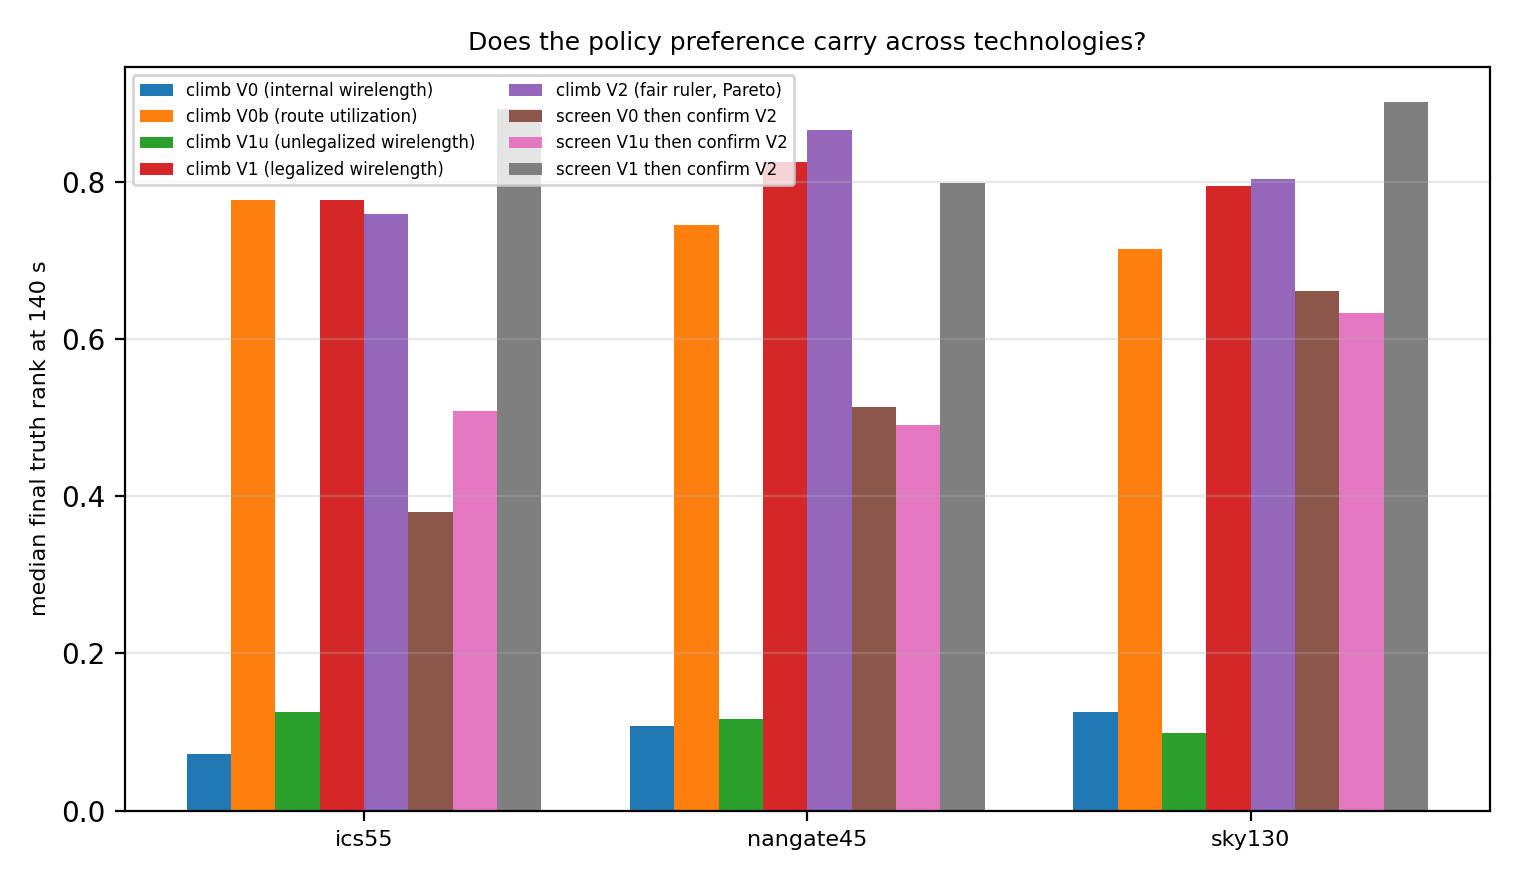
\includegraphics[width=0.9\linewidth]{figures/fig8_transfer.png}
\caption{Policy performance by process technology. The ordering of policies is
preserved; the pre-legalization policies are worst everywhere.}
\end{figure}

\section{Limitations and what we do not claim}

\begin{itemize}
\item We do not claim that accelerating self-improvement has been achieved. The loops
here are per-design and share no learned state, so what we measure is the improvement
dynamics of one loop, not the growth of an improver.
\item The top rung of our ladder is a pre-clock-tree timing evaluation with a wireload
model, so it is a rung rather than signoff. Extending to signoff is future work.
\item The transfer arms have four designs each, so the transfer correlations are
reported as an ordering rather than as precise coefficients, and the timing rung does
not resolve on those technologies, so transfer is measured on the geometry ruler.
\item We do not claim to beat commercial tools in absolute quality; our absolute
numbers are modest and the external reference is an anchor for a relative comparison.
\item The host was shared and heavily loaded during part of the campaign, so wall-clock
cost records are noisy; the per-stage CPU costs are recorded alongside and are stable.
\item The signoff comparison is one design and two candidates (\S5.5), included as
an illustration that the ordering survives to the end of the flow. It is not a
sampling measurement and no other claim depends on it.
\end{itemize}

\section{Conclusion}

A verifier is not a noisy version of the truth. The signal that is cheapest to compute
and most natural to optimize --- the wirelength reported before legalization --- is
anti-correlated with the truth and with the rung above it. Selecting on it costs about
$20\%$ of wirelength and $125\%$ of congestion, and the choice it makes is visibly
worse on an external commercial yardstick on 31 of 32 designs. A self-improvement loop
driven by such a verifier does not plateau; it goes backwards while reporting progress:
across 800 trajectories the cheap loops ended half a pool-step worse than they started
in $90$--$93\%$ of runs while reporting a believed improvement of $+1.22$ rank points,
with a true-improvement horizon of $r^\star=0$.

The practical consequence is a rule with a measured margin: pay for the cheapest
verifier that preserves the truth ordering, use it to screen for breadth, and confirm
the survivors with the strongest available one. That policy beat the best fixed-rung
strategy at every budget tested, by roughly nine rank points, and its preference order
transferred across process technologies with rank correlation $0.87$--$0.91$. Ranking
candidates on an unfaithful verifier was worse than not screening at all.

The mechanism is measurable rather than inferred: splitting every accepted edit into
confirmed gain and harmful loss shows the damage term is $3.4$ times the gain term for
the cheap rungs, with the relation reversed for the faithful ones. A weak verifier is not
merely more permissive, it lets through more edits of worse quality, and the damage is
written into the persistent state and then built upon. That is why it produces a ceiling
rather than noise.

The findings survive leaving the designs that produced them: on six sealed designs, used
for nothing except the report, the unfaithful arm is negative at $-0.54$ and the faithful
arms positive, as on the development split; the eight out-of-distribution designs repeat
the pattern; and a live implementation driving real placements each round reproduces the
rung ordering, the sign and the horizon.

Three things we do not claim. We did not achieve accelerating self-improvement: the
loops here are per-design and share no learned state, so what we measure is the dynamics
of one loop, not the growth of an improver. The timing evidence is a pre-clock-tree
evaluation with a wireload model, so even the top of our ladder is a rung rather than
signoff. And the signoff comparison is one design and two candidates, an illustration
rather than a sampling measurement.

What the work contributes is the instrument and the discipline to use it: the ladder,
the cost ledger, the external anchor, the frozen protocol and the seven dated
amendments, each recording a defect that produced results which looked plausible rather
than results which broke. The campaign also produced its own illustration of the thesis:
a preliminary conclusion in this study, drawn on a pool one third the size, was wrong,
and was corrected by the same rule the paper recommends --- measure with a stronger
verifier than the one that produced the claim.

\appendix
\section{Protocol, artifacts and reproducibility}

Every number in this paper is produced by a script in \texttt{ieda/rsi/analysis} from
an append-only ledger in which each record carries a protocol hash. The protocol and its
seven amendments are frozen by hash and the runner refuses to start if the protocol hash
does not match. Measurements are keyed on the candidate and the solver binary rather than
on the experiment that requested them, so re-running the analyses is exact and re-running
experiments reuses every valid measurement. A single audit script,
\texttt{analysis/number\_audit.py}, re-derives every number quoted here from the frozen
analysis output and compares it with the value in the text; it reports 42 checks and all
of them pass.

\begin{center}
\begin{tabular}{ll}
\toprule
artifact & path \\
\midrule
protocol and amendments & \texttt{ieda/rsi/protocol/} \\
leveled verifier and ledger & \texttt{ieda/rsi/harness/} \\
analyses and figures & \texttt{ieda/rsi/analysis/} \\
number index (number, script, status) & \texttt{ieda/rsi/paper/RESULTS.md} \\
draft with FINAL/PENDING labels & \texttt{ieda/rsi/paper/DRAFT-v0.1.md} \\
\bottomrule
\end{tabular}
\end{center}

\paragraph{Kill criteria.} Four criteria were registered before measurement (a fifth
concern, whether the conclusions were fitted to the designs that suggested them, is
addressed by the held-out splits in \S7.1 rather than by a criterion). K1 (a
finite horizon exists for weak rungs) passed with $r^\star=0$ for both cheap rungs. K2
(cheap and strong rungs are distinguishable) passed at $|\Delta\rho|>0.5$ spread. K3
(the method beats the best fixed rung at equal cost) passed with a margin of
$+0.071$ to $+0.089$, after an earlier FAIL on a smaller pool. K4 (reproducibility)
passed after the seeding amendment.

\end{document}
